%%%%%%%%%%%%%%%%%%%%%%%%%%%%%%%%%%%%%%%%%%%%%%%%%%%%%%%%%%%%%%%%%%%%%%%%%%%%%%%%%%%%%%
% Modelo de relatório de Disciplina de MLP a partir da
% classe latex iiufrgs disponivel em http://github.com/schnorr/iiufrgs
%%%%%%%%%%%%%%%%%%%%%%%%%%%%%%%%%%%%%%%%%%%%%%%%%%%%%%%%%%%%%%%%%%%%%%%%%%%%%%%%%%%%%%

% Ignore o comentario acima e imagine que exista um modelo de relatorio de CCI em algum lugar

%%%%%%%%%%%%%%%%%%%%%%%%%%%%%%%%%%%%%%%%%%%%%%%%%%%%%%%%%%%%%%%%%%%%%%%%%%%%%%%%%%%%%%
% Definição do tipo / classe de documento e estilo usado
%%%%%%%%%%%%%%%%%%%%%%%%%%%%%%%%%%%%%%%%%%%%%%%%%%%%%%%%%%%%%%%%%%%%%%%%%%%%%%%%%%%%%%
%
\documentclass{iiufrgs}

%%%%%%%%%%%%%%%%%%%%%%%%%%%%%%%%%%%%%%%%%%%%%%%%%%%%%%%%%%%%%%%%%%%%%%%%%%%%%%%%%%%%%%
% Importação de pacotes
%%%%%%%%%%%%%%%%%%%%%%%%%%%%%%%%%%%%%%%%%%%%%%%%%%%%%%%%%%%%%%%%%%%%%%%%%%%%%%%%%%%%%%
% (a A seguir podem ser importados os pacotes necessários para o documento, de acordo 
% com a necessidade)
%
\usepackage[brazilian]{babel}	    % para texto escrito em pt-br
\usepackage[utf8]{inputenc}         % pacote para acentuação
\usepackage{graphicx}         	    % pacote para importar figuras
\usepackage[T1]{fontenc}            % pacote para conj. de caracteres correto
\usepackage{times}                  % pacote para usar fonte Adobe Times
\usepackage{enumerate}              % para lista de itens com letras
\usepackage{breakcites}
\usepackage{tikz}
\usepackage[oldvoltagedirection]{circuitikzgit}
\usepackage{caption}
\usepackage{siunitx}
\usepackage{placeins}
\usepackage{titlesec}
\usepackage{enumitem}
\usepackage{titletoc}
\usepackage{subfig}
%\usepackage{listings}			    % para listagens de código-fonte
\usepackage{mathptmx}               % p/ usar fonte Adobe Times nas formulas matematicas
\usepackage{url}                    % para formatar URLs
%\usepackage{color}				    % para imagens e outras coisas coloridas
\usepackage{fixltx2e}              % para subscript
%\usepackage{amsmath}               % para \epsilon e matemática
%\usepackage{amsfonts}
%\usepackage{setspace}			    % para mudar espaçamento dos parágrafos
%\usepackage[table,xcdraw]{xcolor}  % para tabelas coloridas
%\usepackage{longtable}             % para tabelas compridas (mais de uma página)
%\usepackage{float}
%\usepackage{booktabs}
\usepackage{tabularx}
%\usepackage{hyperref}

\usepackage[alf,abnt-emphasize=bf]{abntex2cite}	% pacote para usar citações abnt

%%%%%%%%%%%%%%%%%%%%%%%%%%%%%%%%%%%%%%%%%%%%%%%%%%%%%%%%%%%%%%%%%%%%%%%%%%%%%%%%%%%%%%
% Macros, ajustes e definições
%%%%%%%%%%%%%%%%%%%%%%%%%%%%%%%%%%%%%%%%%%%%%%%%%%%%%%%%%%%%%%%%%%%%%%%%%%%%%%%%%%%%%%
%

% define estilo de parágrafo para citação longa direta:
\newenvironment{citacao}{
    %\singlespacing
    %\footnotesize
    \small
    \begin{list}{}{
        \setlength{\leftmargin}{4.0cm}
        \setstretch{1}
        \setlength{\topsep}{1.2cm}
        \setlength{\listparindent}{\parindent}
    }
    \item[]}{\end{list}
}

% adiciona a fonte em figuras e tabelas
\newcommand{\fonte}[1]{\\Fonte: {#1}}

\newcommand{\virtuoso}{\textit{Virtuoso}}

\newcommand{\titlepagespecificinfo}{Relatório apresentado como requisito parcial para a obtenção de conceito na Disciplina de Concepção de Circuitos Integrados.}
% \def\@cipspecificinfo{Concepção de Circuitos Integrados}


% Ative o seguinte caso alguma nota de rodapé fique muito longa e quebre entre múltiplas
% páginas
%\interfootnotelinepenalty=10000

%%%%%%%%%%%%%%%%%%%%%%%%%%%%%%%%%%%%%%%%%%%%%%%%%%%%%%%%%%%%%%%%%%%%%%%%%%%%%%%%%%%%%%
% Informações gerais                                   
%%%%%%%%%%%%%%%%%%%%%%%%%%%%%%%%%%%%%%%%%%%%%%%%%%%%%%%%%%%%%%%%%%%%%%%%%%%%%%%%%%%%%%

% título
\title{RELATÓRIO 2} 

% autor
%\author{Autores(s)}{Aluno(s)} % {sobrenome}{nome}
\author{Silva}{Henrique Corrêa Pereira da}

% Professor orientador da disciplina
\advisor[Prof.~Dr.]{Augusto da Luz Reis}{Ricardo}

% Nome do(s) curso(s):
\course{Curso de Graduação em Ciência da Computação}

% local da realização do trabalho 
\location{Porto Alegre}{RS} 

% data da entrega do trabalho (mês e ano)
\date{5}{2018}


% Palavras chave
\keyword{CCI}
\keyword{Virtuoso}
\keyword{Inversor}
\keyword{Relatório}


%%%%%%%%%%%%%%%%%%%%%%%%%%%%%%%%%%%%%%%%%%%%%%%%%%%%%%%%%%%%%%%%%%%%%%%%%%%%%%%%%%%%%%
% Início do documento e elementos pré-textuais
%%%%%%%%%%%%%%%%%%%%%%%%%%%%%%%%%%%%%%%%%%%%%%%%%%%%%%%%%%%%%%%%%%%%%%%%%%%%%%%%%%%%%%

% Declara início do documento
\begin{document}

% inclui folha de rosto 
\maketitle

\selectlanguage{brazilian}

% Sumario
\tableofcontents



%%%%%%%%%%%%%%%%%%%%%%%%%%%%%%%%%%%%%%%%%%%%%%%%%%%%%%%%%%%%%%%%%%%%%%%%%%%%%%%%%%%%%
% Aqui comeca o texto propriamente dito
%%%%%%%%%%%%%%%%%%%%%%%%%%%%%%%%%%%%%%%%%%%%%%%%%%%%%%%%%%%%%%%%%%%%%%%%%%%%%%%%%%%%%

%espaçamento entre parágrafos
%\setlength{\parskip}{6 pt}

\selectlanguage{brazilian}

%%%%%%%%%%%%%%%%%%%%%%%%%%%%%%%%%%%%%%%%%%%%%%%%%%%%%%%%%%%%%%%%%%%%%%%%%%%%%%%%%%%%%
% Introdução
%

%Este capítulo tem o objetivo de descrever os detalhes necessários à correta formatação do documento. As informações aqui apresentadas devem ser suficientes para formatar corretamente o documento no ambiente \LaTeX.

%Os \textbf{Capítulos} são sempre iniciados com o comando \texttt{\char'134chapter}, que coloca-os em uma nova folha, em letras maiúsculas, numerados e  alinhados à esquerda. Para os \textbf{capítulos não-numerados} (Listas, Resumo, Abstract, Referências, etc.), o título é centralizado na linha Para tanto, usar o comando \texttt{\char'134chapter*}. Para ambos, são deixados 90 pt de espaçamento anterior (ou seja, distância da margem superior) e 42 pt de espaçamento posterior (espaço até o início do texto ou primeira subdivisão). 

%Todos os \textbf{demais parágrafos de texto} são escritos em espaçamento simples, com observância de 6 pt de espaçamento em relação ao parágrafo seguinte. O estilo atual já considera essas retrições. 


%As demais subdivisões do texto (seções, subseções, etc.) são formatadas com o título alinhado sempre à esquerda, precedido da respectiva numeração. Para tanto, no \LaTeX, você deve utilizar os comandos \texttt{\char'134section},  \texttt{\char'134subsection} e  \texttt{\char'134subsubsection}.

%São permitidas subdivisões até o 5º nível (onde o capítulo é o 1º. nível), porém no sumário inclui-se somente os títulos até o nível 3\footnote{O formato adotado pela ABNT prevê apenas três níveis (capítulo, seção e subseção).}. Assim, \texttt{\char'134subsubsection} não é aconselhado. 


%%%%%%%%%%%%%%%%%%%%%%%%%%%%%%%%%%%%%%%%%%%%%%%%%%%%%%%%%%%%%%%%%%%%%%%%%%%%%%%%%%%%%
% Visao Geral
%

\chapter{Introdução}\label{intro}

Neste relatório, construiremos leiautes e esquemáticos de células NAND2 e NOR2 e observaremos suas performances utilizando as  seguintes métricas:

\begin{enumerate}[leftmargin=3em, noitemsep] % [label={--}]
    \setlength{\itemindent}{1em}
    \item T\textsubscript{lh}: tempo de subida do sinal;
    \item T\textsubscript{hl}: tempo de descida do sinal;
    \item Tp\textsubscript{lh}: tempo de propagação \textit{low-high}; 
    \item Tp\textsubscript{hl}: tempo de propagação \textit{high-low}; 
    \item Tp\textsubscript{médio}: tempo de propagação médio; 
    \item P\textsubscript{média}: potência média das células; 
    \item P\textsubscript{RMS}: potência \textit{RMS} das células.
\end{enumerate}

Além disso, será feita a análise \textit{Layout versus Schematic} para cada célula a fim de  verificar a funcionalidade do leiaute contra o esquemático. Mais detalhes sobre a implementação das portas lógicas e do circuito no Capítulo \ref{proposta}. \

\begin{figure}[htb]
    \centering
    \caption{Circuito NAND2 a ser projetado.}
    \label{fig:nand2}
    \begin{circuitikz}
        \node [american nand port] (nand) at (5, 2) {};
        \path (nand.in 1) -- ++(-3, 0) node (source1) {};
        \path (nand.in 2) -- ++(-0.7, 0) node (source2) {};
        \path (source1) -- ++(0, -2.3) node (gnd1) {};
        \path (gnd1) -- ++(2.3, 0) node (gnd2) {};
        \path (gnd1) -- ++(5.5, 0) node (gnd3) {};
        \path (gnd3) -- ++(0, 2.02) node (out) {};
        \node [ground] at (gnd1) {};
        \node [ground] at (gnd2) {};
        \node [ground] at (gnd3) {};

        \draw (gnd1) to[vsourcesquare, v=$3.3 V$] (source1);
        \draw (gnd2) to[vsourcesquare, v=$3.3 V$] (source2);
        \draw (source1) to[short] (nand.in 1);
        \draw (source2) to[short] (nand.in 2);
        \draw (nand.out) to[short] (out);
        \draw (gnd3) to[pC, l_=$50fF$] (out);
        \node at (0, 3.2) {};
    \end{circuitikz}
\end{figure}

\begin{figure}[htb]
    \centering
    \caption{Circuito NOR2 a ser projetado.}
    \label{fig:nor2}
    \begin{circuitikz}
        \node [american nor port] (nor) at (5, 2) {};
        \path (nor.in 1) -- ++(-3, 0) node (source1) {};
        \path (nor.in 2) -- ++(-0.7, 0) node (source2) {};
        \path (source1) -- ++(0, -2.3) node (gnd1) {};
        \path (gnd1) -- ++(2.3, 0) node (gnd2) {};
        \path (gnd1) -- ++(5.5, 0) node (gnd3) {};
        \path (gnd3) -- ++(0, 2.02) node (out) {};
        \node [ground] at (gnd1) {};
        \node [ground] at (gnd2) {};
        \node [ground] at (gnd3) {};

        \draw (gnd1) to[vsourcesquare, v=$3.3 V$] (source1);
        \draw (gnd2) to[vsourcesquare, v=$3.3 V$] (source2);
        \draw (source1) to[short] (nor.in 1);
        \draw (source2) to[short] (nor.in 2);
        \draw (nor.out) to[short] (out);
        \draw (gnd3) to[pC, l_=$50fF$] (out);
        \node at (0, 3.2) {};
    \end{circuitikz}
\end{figure}

\chapter{Proposta}\label{proposta}
A proposta do relatório é construir e realizar a medição de métricas de implementações das portas lógicas NAND2 e NOR2 na tecnologia CMOS C35B4 da \textit{Austria Microsystems}, utilizando valores de W\textsubscript{p} e de W\textsubscript{n} dessas respectivas portas conforme a Tabela \ref{tab:imp}.
Além disso, o circuito também deverá seguir às seguintes especificações:

\begin{itemize}[noitemsep]
    \setlength{\itemindent}{1em}
    \item VDD = \SI{3.3}{\V};
    \item $1/{f_1}$ = \SI{10}{\ns};
    \item $1/{f_2}$ = \SI{20}{\ns};
    \item T\textsubscript{rise} = \SI{200}{\ps};
    \item T\textsubscript{fall} = \SI{200}{\ps};
    \item P1\textsubscript{width} = \SI{5}{\ns};
    \item P2\textsubscript{width} = \SI{10}{\ns}.
\end{itemize}

Criados os leiautes, é obrigatório tanto o teste individual de cada um utilizando as ferramentas \textit{DRC} e \textit{LVS} quanto a extração das capacitâncias parasitas de cada implementação.

\begin{table}[ht]
    \centering
    \caption{Dimensões em cada implementação.}
    \label{tab:imp}
    \begin{tabular}{l c c}
        \hline
        Implementação
        & W\textsubscript{p}
        & W\textsubscript{n} \\ \hline
        NAND2 & \SI{3.0}{\um}   & \SI{2.0}{\um}     \\ 
        NOR2 & \SI{4.0}{\um}    & \SI{1.0}{\um}     \\ \hline
    \end{tabular}
\end{table}

\chapter{Análise}\label{analise}
Neste capítulo abordaremos cada implementação do inversor e, no Capítulo \ref{resultados}, analisaremos os resultados e faremos algumas observações sobre o circuito simulado.

A Figura \ref{fig:both} mostra o esquemático de ambas portas estáticas CMOS que implementaremos.

\begin{figure}[htbp]
    \centering
    \caption{Esquemático de ambas NOR2 e NAND2 em CMOS.}
    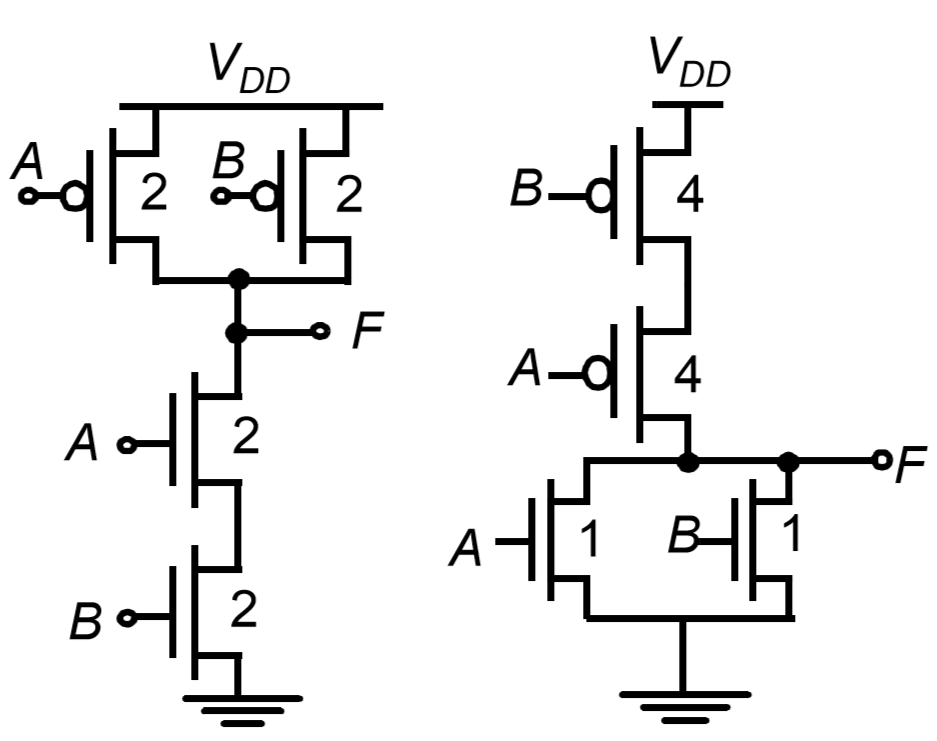
\includegraphics[scale=0.6]{images/schem_both.png}
    \label{fig:both}
\end{figure}

\section{NAND2}\label{nand}
A NAND2, como vista anteriormente na Aula Prática 3, possui transistores PMOS e NMOS dimensionados respectivamente em \SI{3.0}{\um} e \SI{2.0}{\um}, e, assim como na aula prática, as células projetadas tem \SI{14}{\um} de altura num processo CMOS de substrato P\textsuperscript{-}.

A Figura \ref{fig:esquematico-nand} mostra o esquemático da porta lógica na ferramenta \virtuoso, e a Figura \ref{fig:leiaute-nand} mostra o seu respectivo leiaute. O leiaute foi feito manualmente sem utilizar as ferramentas de automação e de simplificação do processo de criação de leiaute do \virtuoso.

\begin{figure}[htbp]
    \centering
    \caption{Esquemático da NAND2}
    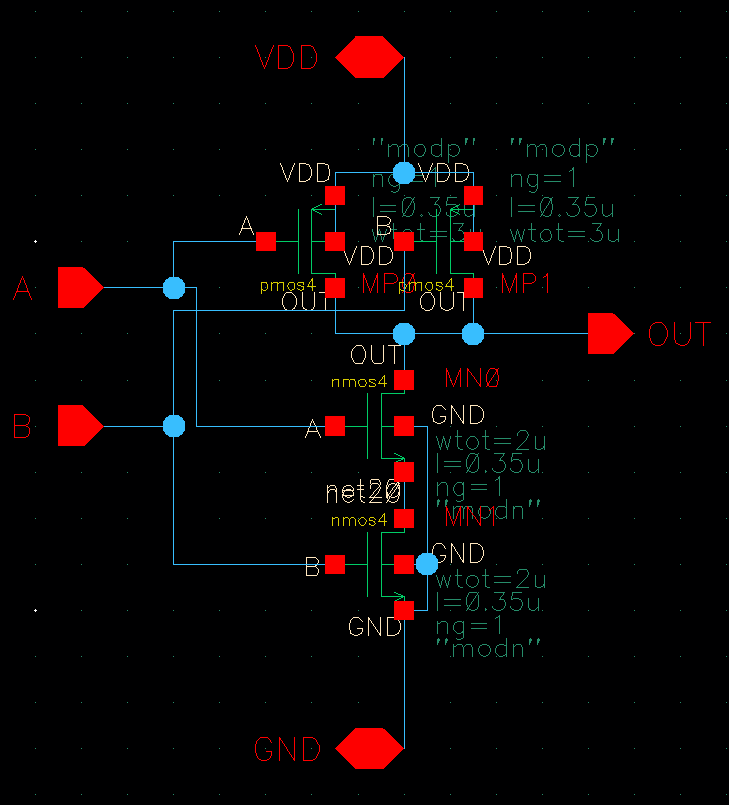
\includegraphics[scale=0.8]{images/schem_nand.png}
    \label{fig:esquematico-nand}
\end{figure}

\begin{figure}[htbp]
    \centering
    \caption{Leiaute da NAND2}
    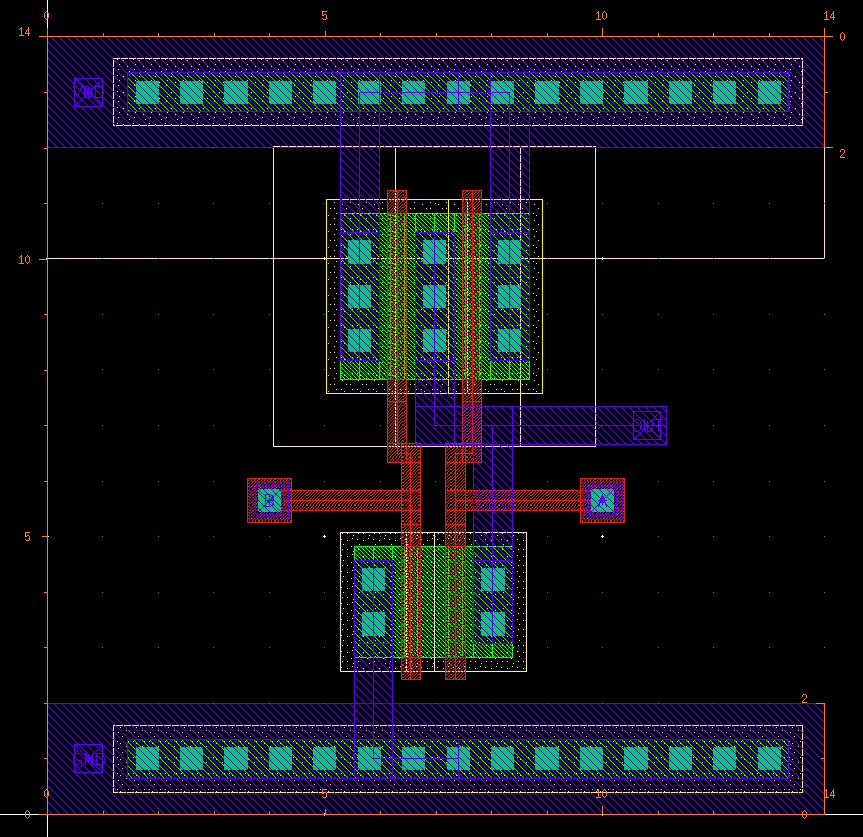
\includegraphics[scale=0.7]{images/layout_nand.png}
    \label{fig:leiaute-nand}
\end{figure}

\FloatBarrier

Os resultados da análise transiente desse circuito estão no Capítulo \ref{resultados}.\

A Figura \ref{fig:trans-nand} mostra o esquemático do circuito na ferramenta \virtuoso, e a Figura \ref{fig:wave-nand} mostra o \textit{waveform} da simulação transiente do circuito.\

\begin{figure}[htbp]
    \centering
    \caption{Esquemático da simulação da transiente da porta.}
    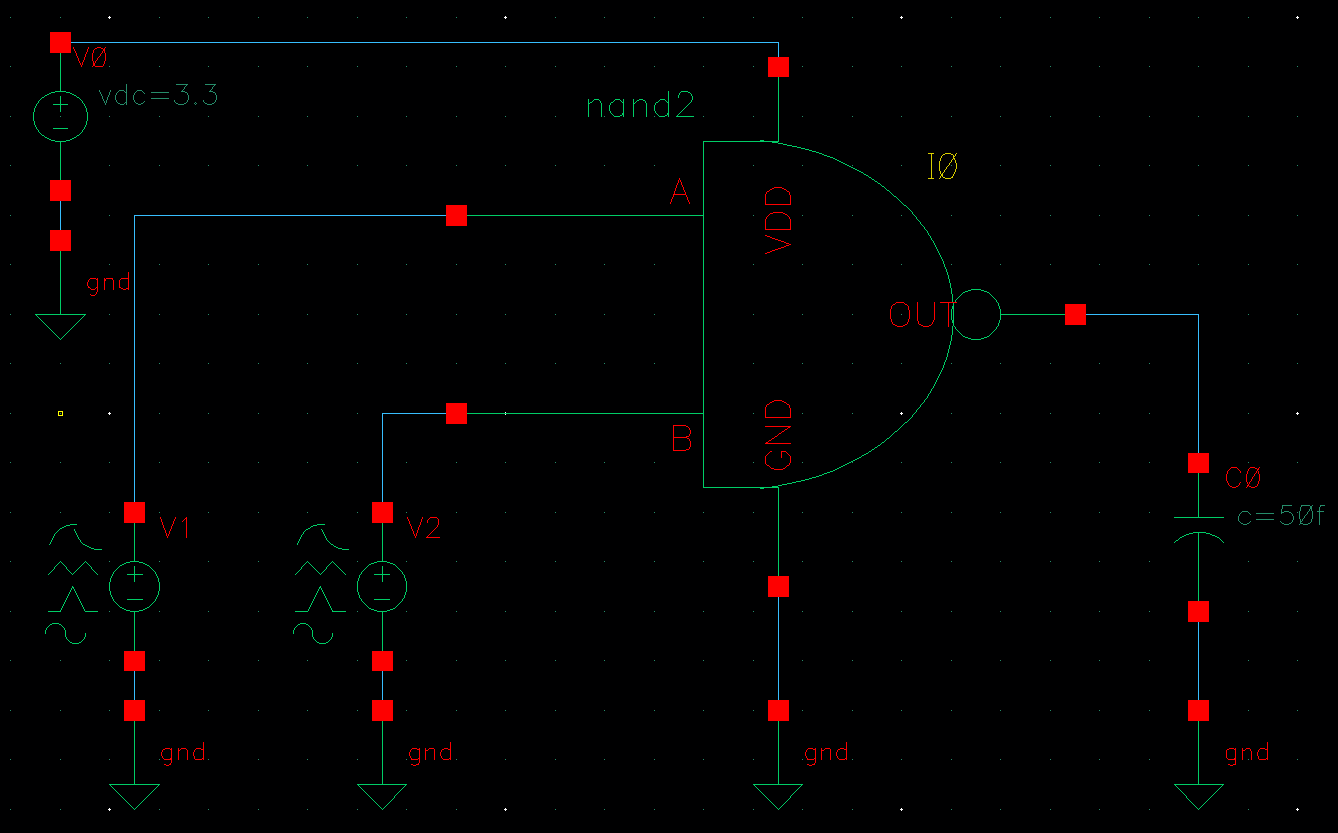
\includegraphics[scale=0.45]{images/schem_trans_nand.png}
    \label{fig:trans-nand}
\end{figure}

\begin{figure}[htbp]
    \centering
    \caption{Waveforms da simulação transiente da porta.}
    \subfloat[united]{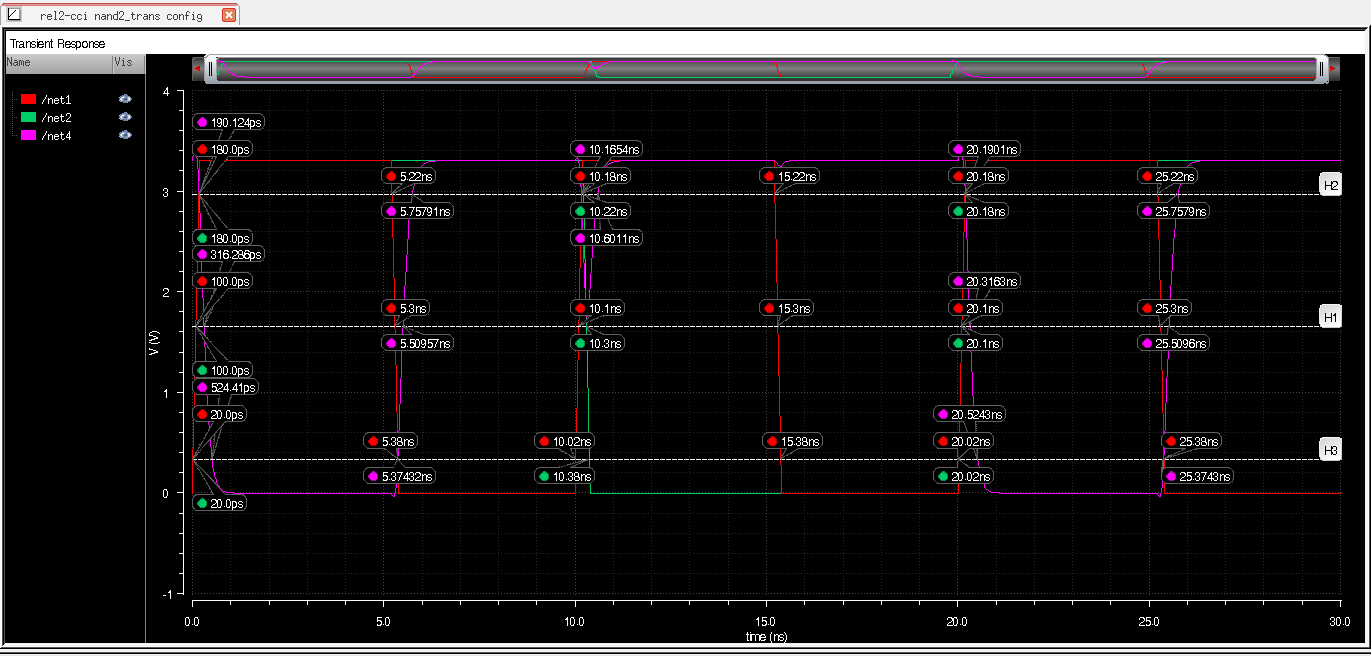
\includegraphics[scale=0.45]{images/wave_nand.png}} \\
    \subfloat[separated]{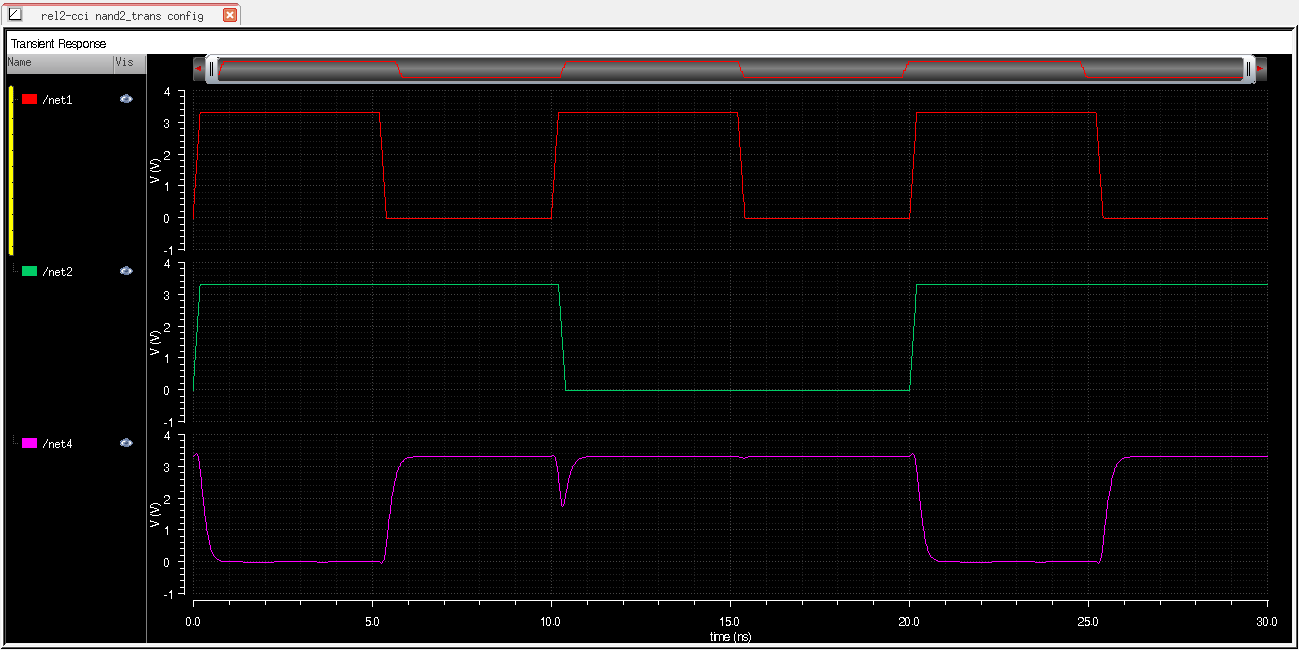
\includegraphics[scale=0.45]{images/wave_sep_nand.png}}
    \label{fig:wave-nand}
\end{figure}

\FloatBarrier

\section{NOR2}\label{nor}
A NOR2, como vista anteriormente na Aula Prática 3, possui transistores PMOS e NMOS dimensionados respectivamente em \SI{4.0}{\um} e \SI{1.0}{\um}, e, assim como na aula prática, as células projetadas tem \SI{14}{\um} de altura num processo CMOS de substrato P\textsuperscript{-}.

A Figura \ref{fig:esquematico-nor} mostra o esquemático da porta lógica na ferramenta \virtuoso, e a Figura \ref{fig:leiaute-nor} mostra o seu respectivo leiaute. O leiaute foi feito manualmente sem utilizar as ferramentas de automação e de simplificação do processo de criação de leiaute do \virtuoso.

\begin{figure}[htbp]
    \centering
    \caption{Esquemático da NOR2}
    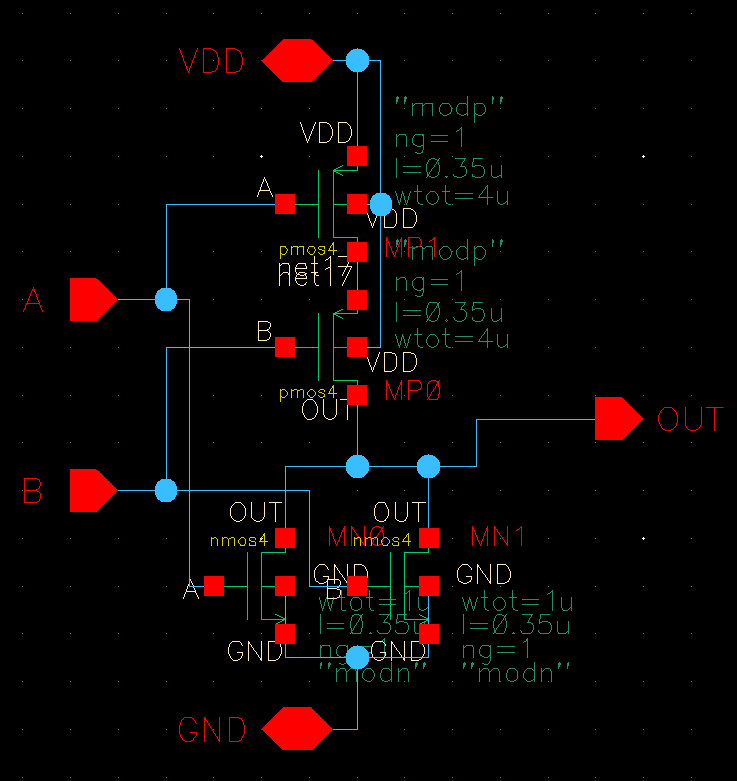
\includegraphics[scale=0.8]{images/schem_nor.png}
    \label{fig:esquematico-nor}
\end{figure}

\begin{figure}[htbp]
    \centering
    \caption{Leiaute da NOR2}
    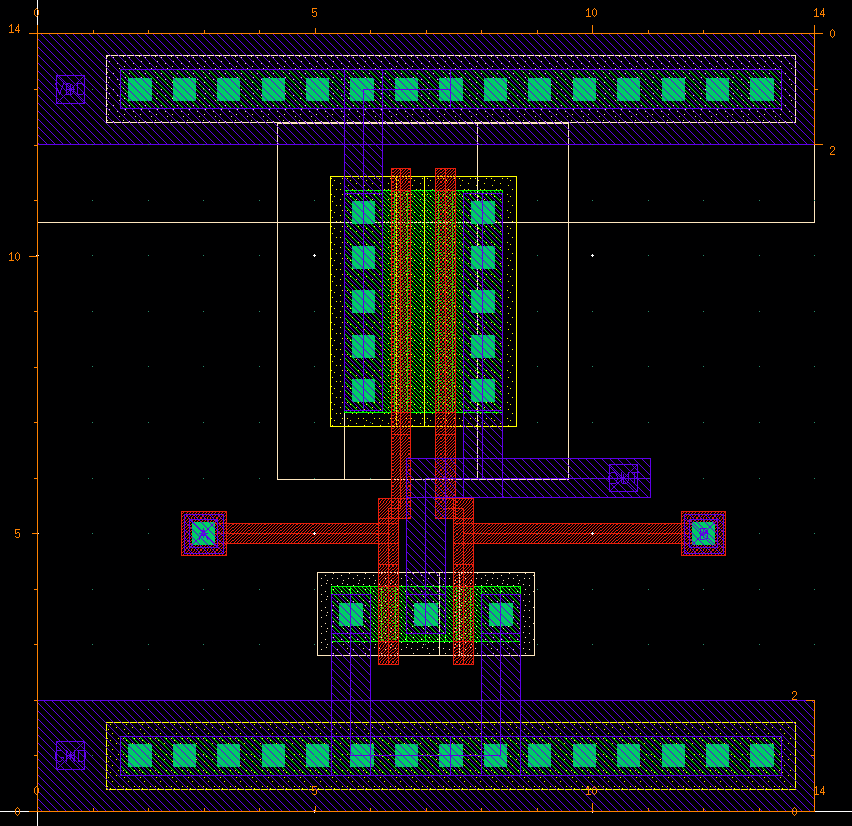
\includegraphics[scale=0.7]{images/layout_nor.png}
    \label{fig:leiaute-nor}
\end{figure}

\FloatBarrier

Os resultados da análise transiente desse circuito estão no Capítulo \ref{resultados}.\

A Figura \ref{fig:trans-nor} mostra o esquemático do circuito na ferramenta \virtuoso, e a Figura \ref{fig:wave-nor} mostra o \textit{waveform} da simulação transiente do circuito.\

\begin{figure}[htbp]
    \centering
    \caption{Esquemático da simulação da transiente da porta.}
    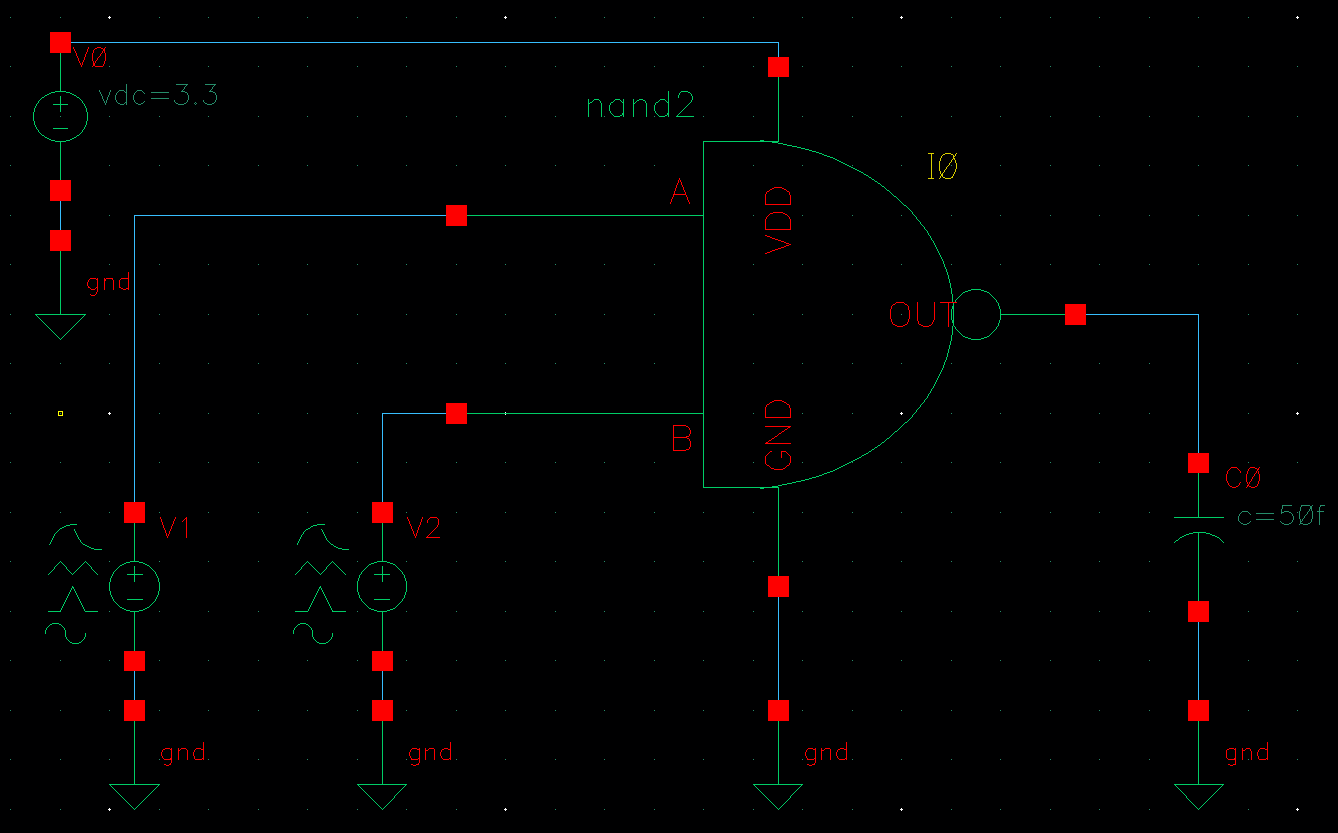
\includegraphics[scale=0.45]{images/schem_trans_nand.png}
    \label{fig:trans-nor}
\end{figure}

\begin{figure}[htbp]
    \centering
    \caption{Waveforms da simulação transiente da porta.}
    \subfloat[united]{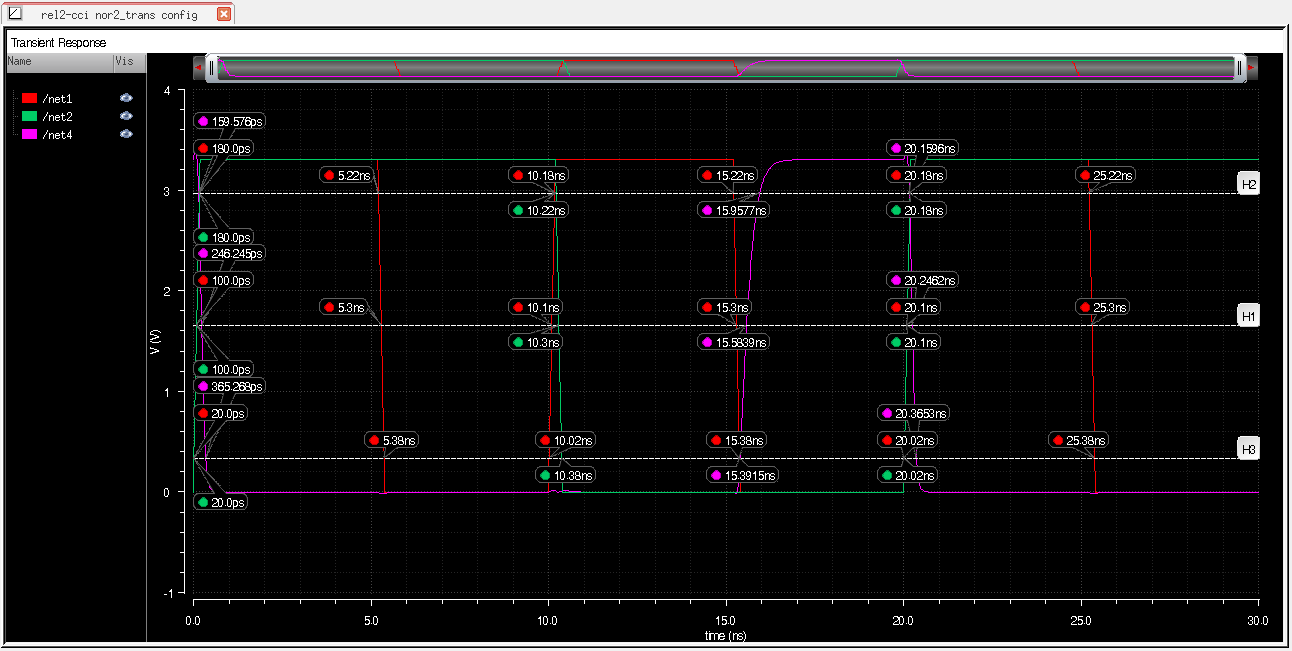
\includegraphics[scale=0.45]{images/wave_nor.png}} \\
    \subfloat[separated]{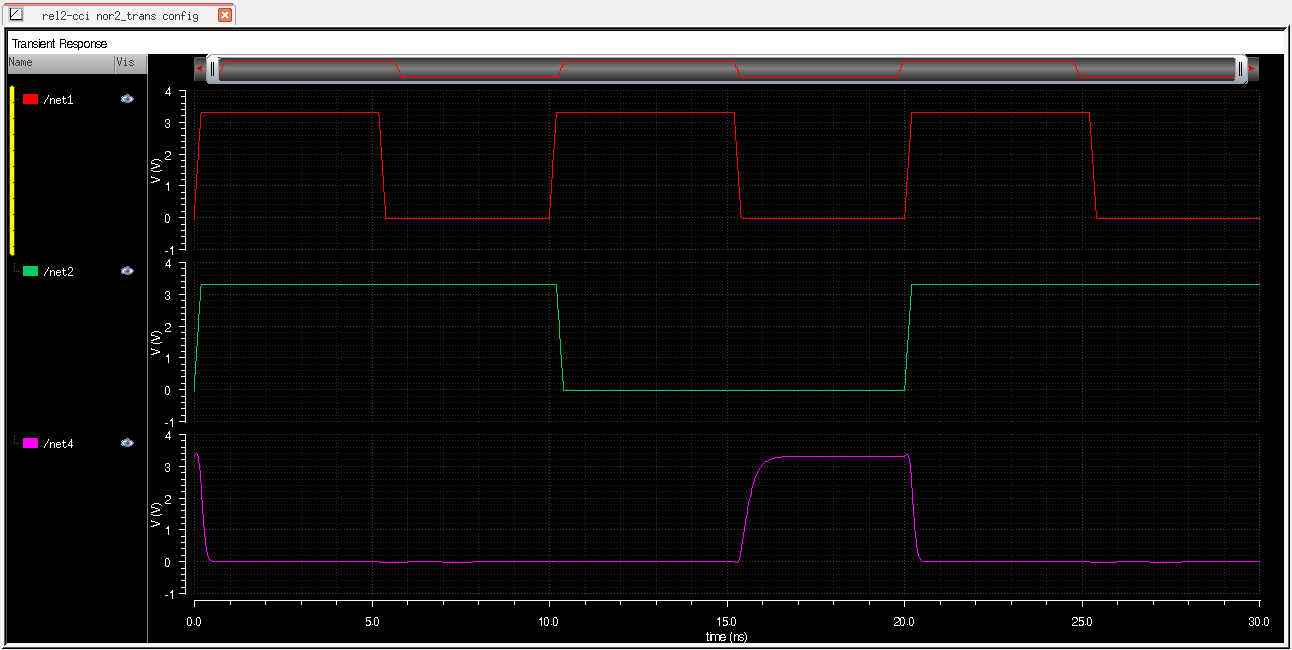
\includegraphics[scale=0.45]{images/wave_sep_nor.png}}
    \label{fig:wave-nor}
\end{figure}

\FloatBarrier

\chapter{Resultados}\label{resultados}
Neste capítulo abordaremos os resultados obtidos nas simulações.

\section{Tabela}\label{tabela}
A Tabela \ref{tab:tempo} define os valores encontrados para cada uma das métricas temporais definidas no Capítulo \nameref{intro} para cada circuito, e a Tabela \ref{tab:potencia} define as métricas de energia para os mesmos ditos circuitos.

\begin{table}[ht]
    \centering
    \caption{Resultados temporais das simulações.}
    \small
    \label{tab:tempo}
    \sisetup{scientific-notation = true, round-mode = places, round-precision = 3}
    \begin{tabular}{l l l l l l}
        \hline
        Porta
        & Tp\textsubscript{HL}
        & Tp\textsubscript{LH}
        & Tp\textsubscript{médio}
        & T\textsubscript{LH}
        & T\textsubscript{HL} \\ \hline
        NAND2
        & \SI{0.209574}{\ns} & \SI{0.21626}{\ns} & \SI{0.212917}{\ns} & \SI{0.383597}{\ns}
        & \SI{0.33421}{\ns} \\
        NOR2
        & \SI{0.28388}{\ns} & \SI{0.14624}{\ns} & \SI{0.21506}{\ns} & \SI{0.56621}{\ns}
        & \SI{0.20571}{\ns} \\
        \hline
    \end{tabular}
\end{table}

\begin{table}[ht]
    \centering
    \caption{Resultados de consumo de potência.}
    \small
    \label{tab:potencia}
    \sisetup{scientific-notation = true, round-mode = places, round-precision = 3}
    \begin{tabular}{l l l}
        \hline
        $\cdots$
        & P\textsubscript{média}
        & P\textsubscript{RMS} \\ \hline
        NAND2
        & \SI{55.94e-6}{\W}  & \SI{264.1e-6}{\W} \\
        NOR2
        & \SI{24.97e-6}{\W} & \SI{163.8e-6}{\W} \\
        \hline
    \end{tabular}
\end{table}

%%%%%%%%%%%%%%%%%%%%%%%%%%%%%%%%%%%%%%%%%%%%%%%%%%%%%%%%%%%%%%

%\bibliographystyle{abntex2-alf}
%\bibliography{biblio} 

\end{document}
